\section{A Beautiful Observation}

This idea occurred to me one day on a public bus in downtown Rochester. Take a function $y = f(x)$ and find one of its values of $x$ that coincides with a minimum of $R(x)$, the radius of curvature for the function. Call that value $x_m$. We know from the theorem is section 9 that the function $y = f(x)$ will spawn a crunch spot from precisely that value of $x$. The crunch spot will occur for the ``critical value'' of $N = \dfrac{f''(x_m)}{|f''(x_m)|}R(x_m)$. But by the definition of radius of curvature, we know that on some potentially small neighborhood of $x_m, y = f(x)$ will approximate an arc of a circle of radius $R(x_m)$ whose center is that crunch spot. Take in your imagination this brief circle arc. If we send forth from each point along that arc a normal line, we know they all converge at the crunch spot. This means no matter what we set $N$ to positive or negative, that the $N$-Units Away Curve spots generated by the part of $y = f(x)$ that approximates a circle will also approximate a circle! This gives us the fascinating result that the ``bottom'' of each divot triangle has a shape approximately a circular arc. This is a very strange, beautiful result and is depicted in Figures $\ref{fig:fig11-38}$ and $\ref{fig:fig11-39}$ bellow:

\begin{figure}[H]
    \centering
    \begin{minipage}[b]{0.9\linewidth}
        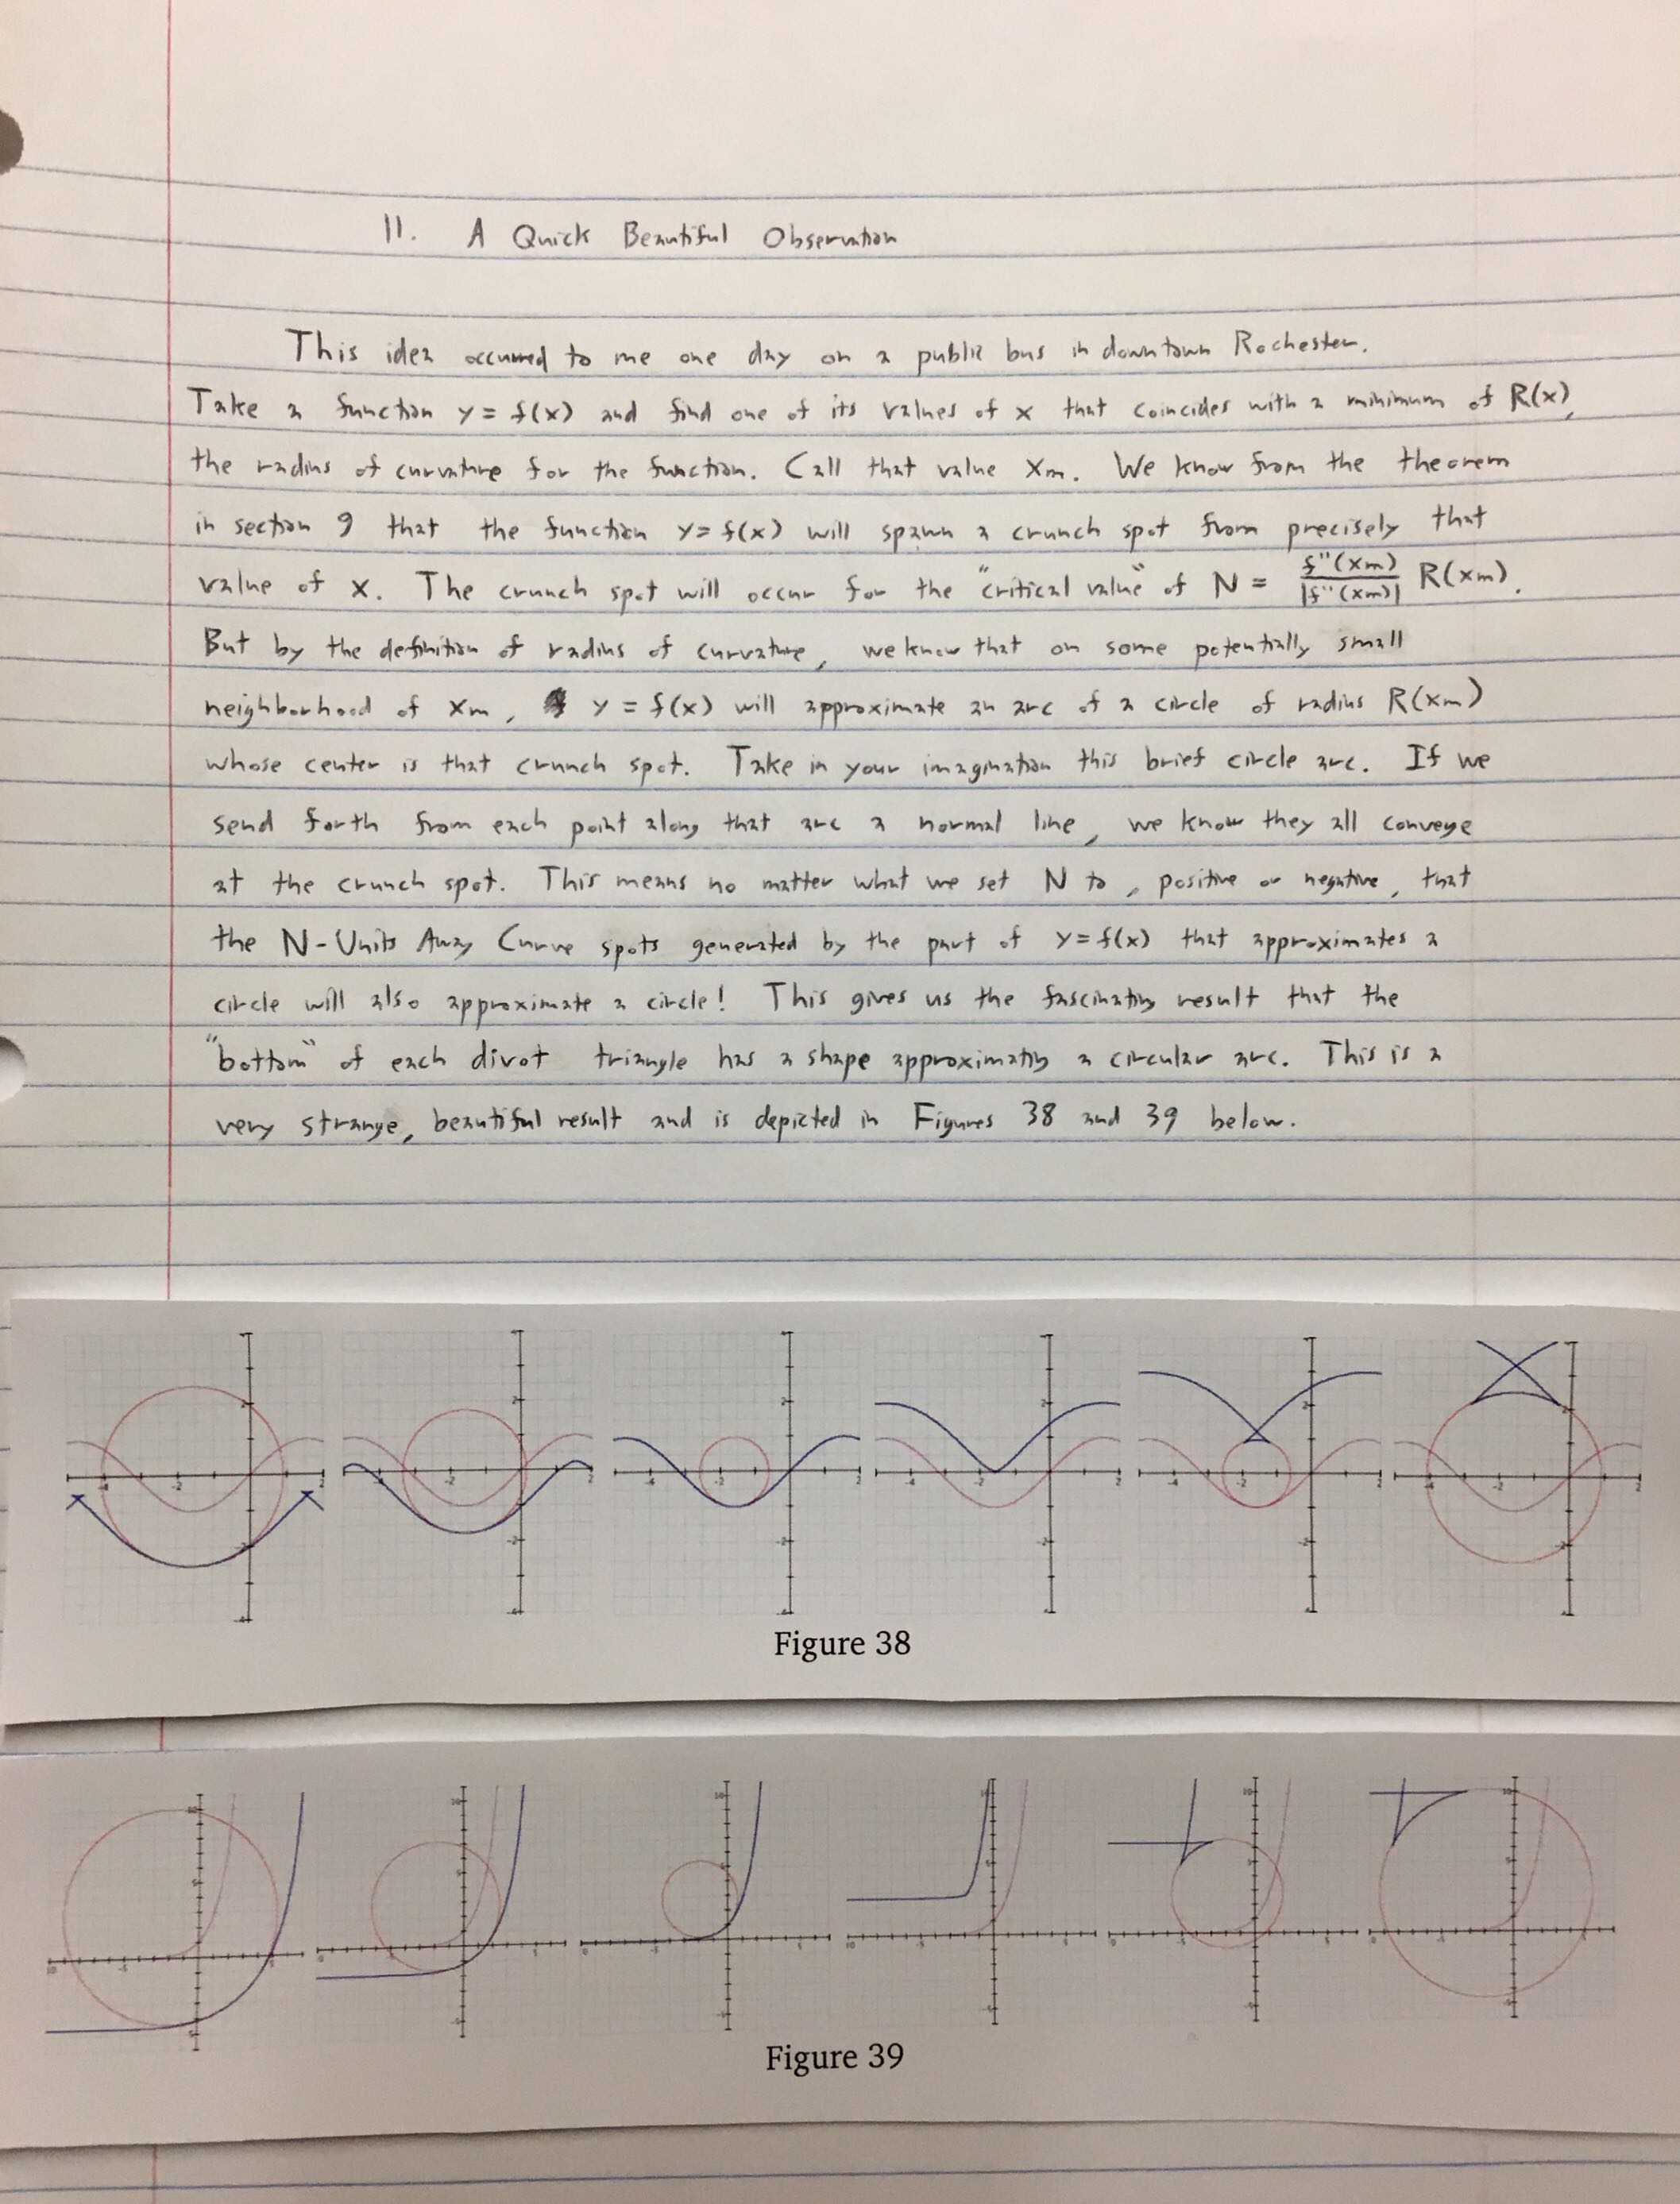
\includegraphics[width = .9\linewidth, height = .25 \textheight, keepaspectratio]{beautiful-observation-img/Fig 11-38.png}
        \caption{Caption}
        \label{fig:fig11-38}
    \end{minipage}
    \begin{minipage}[b]{0.9\linewidth}
        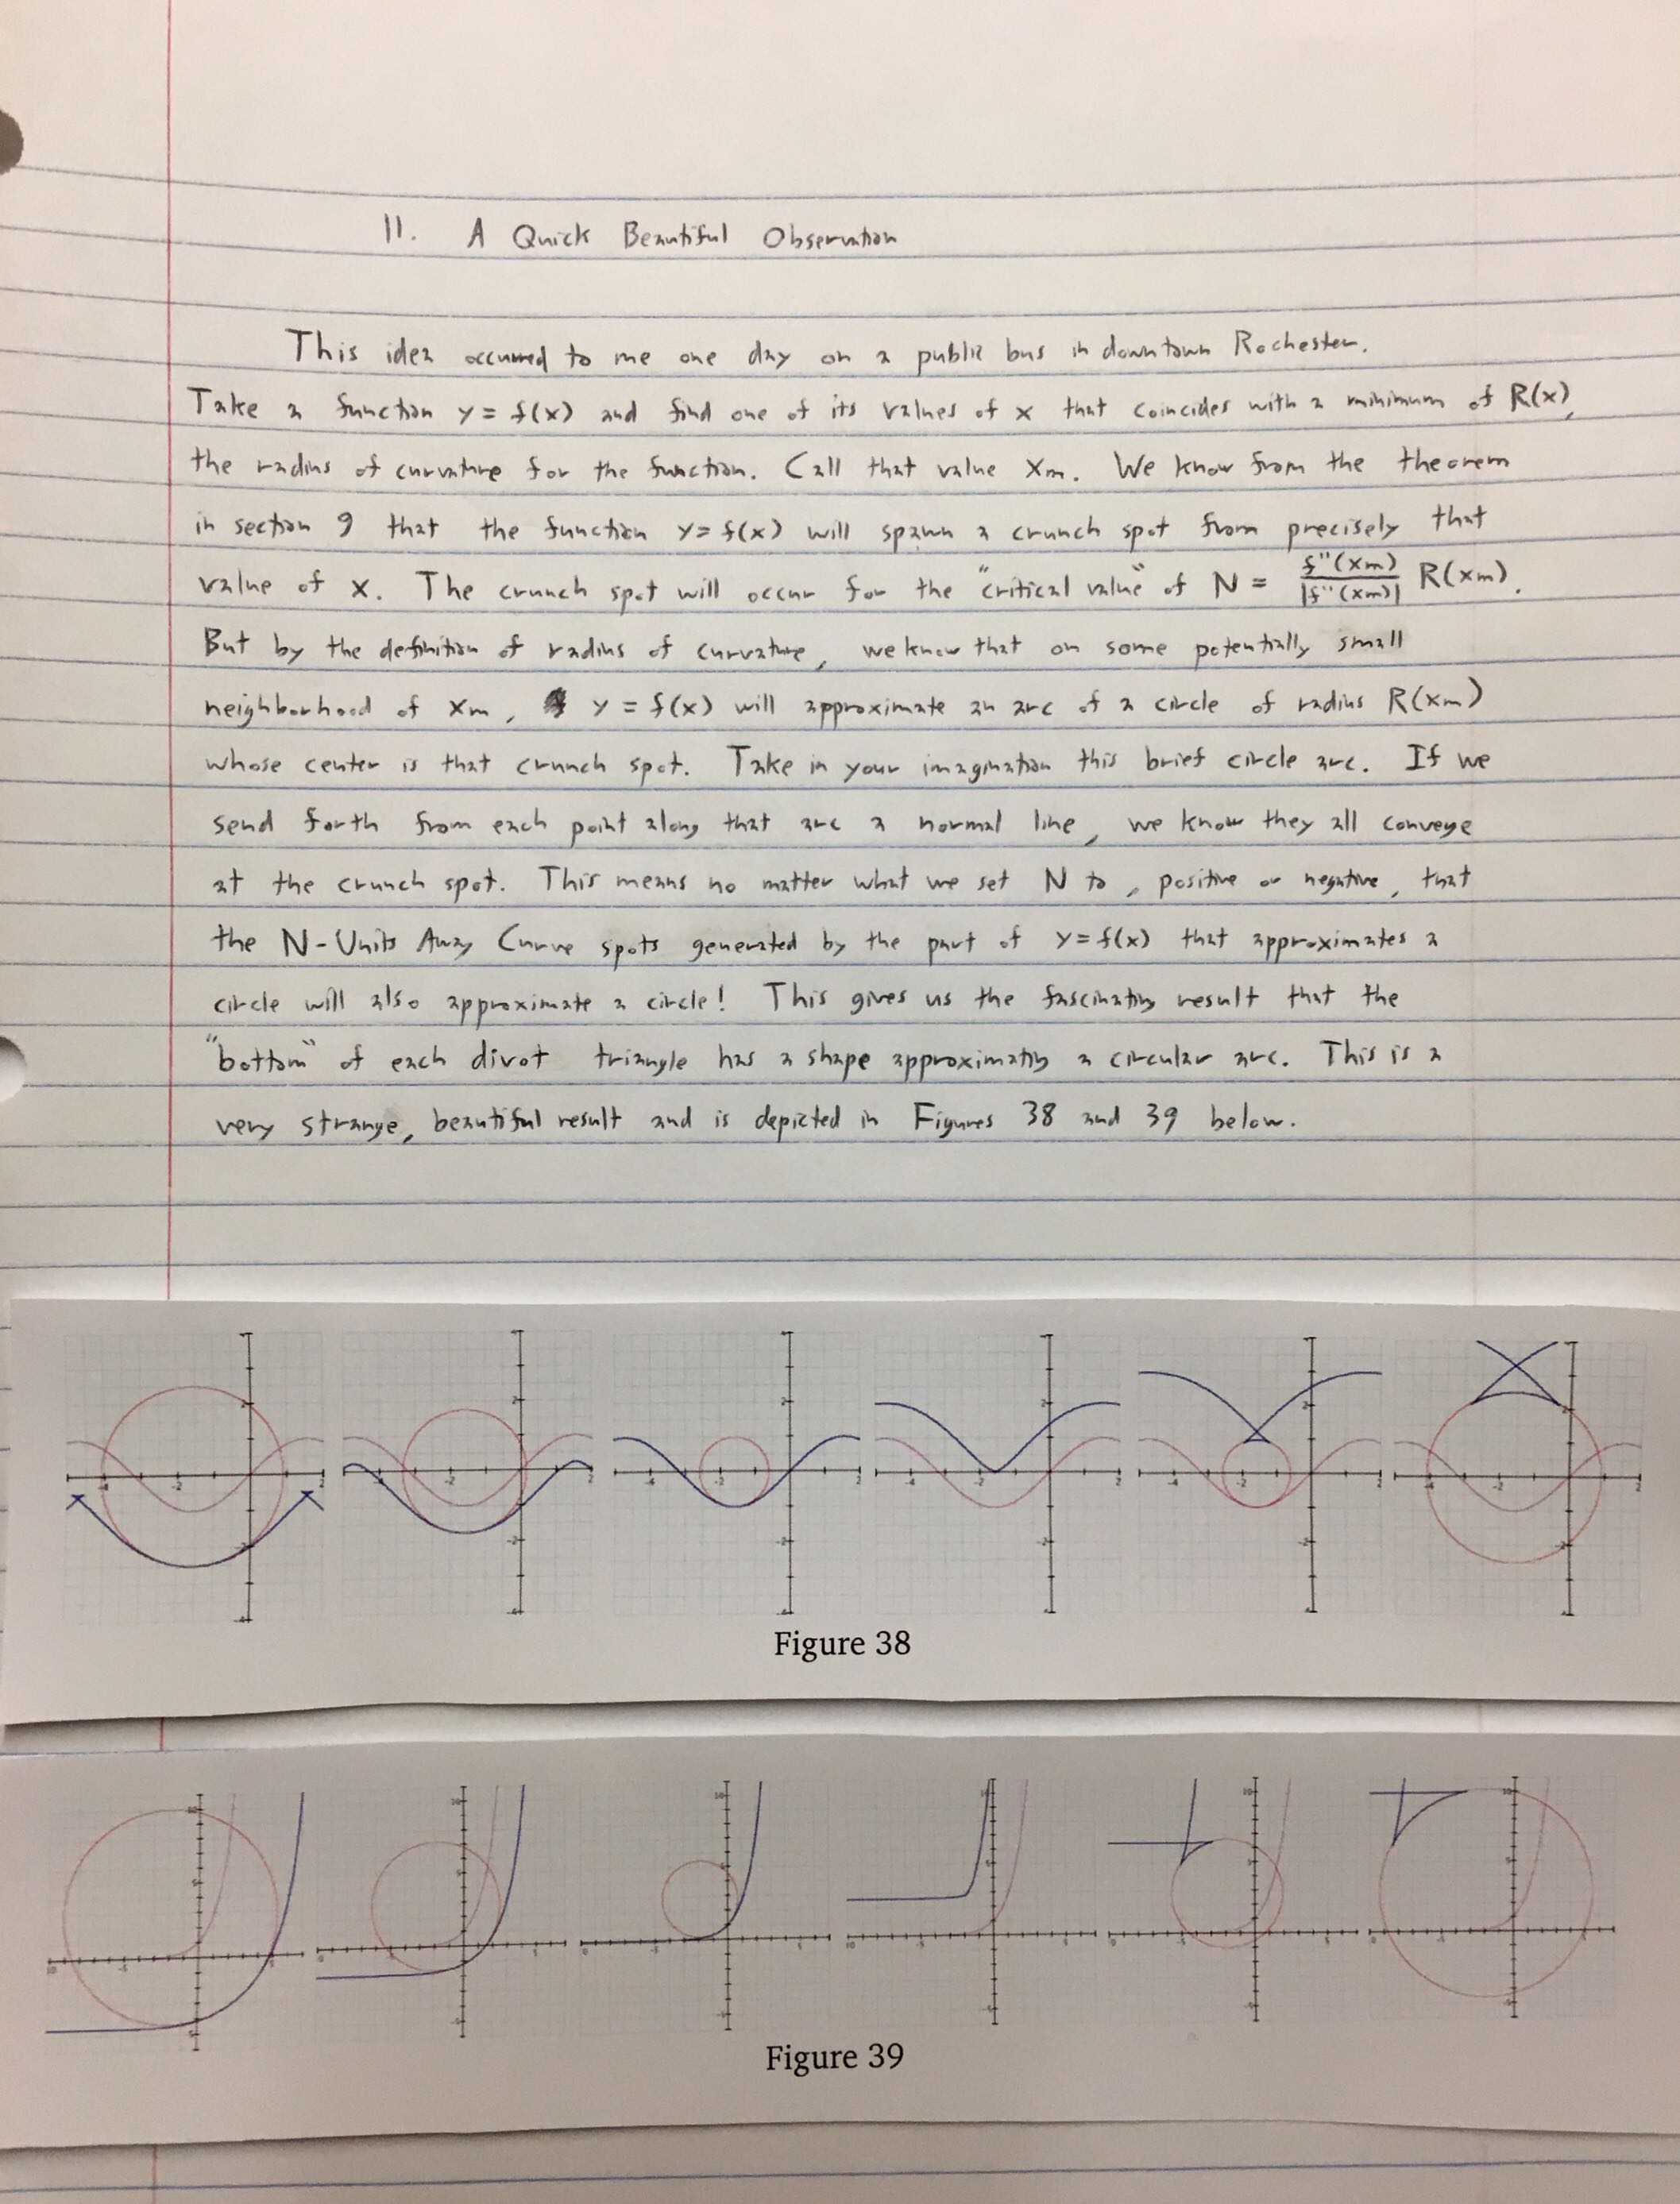
\includegraphics[width = .9\linewidth, height = .25 \textheight, keepaspectratio]{beautiful-observation-img/Fig 11-39.png}
        \caption{Caption}
        \label{fig:fig11-39}
    \end{minipage}
\end{figure}